\FloatBarrier
\begin{figure}[!h]
	\centering
	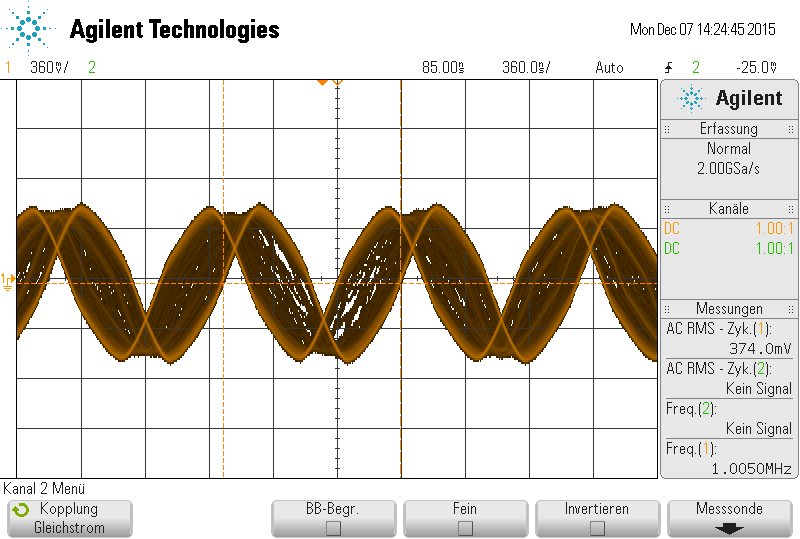
\includegraphics[scale=0.50]{../Grafiken/Messung_d2.png}
	\caption{Darstellung der periodischen Phasenvariation zwischen der modulierten Spannung und der
	Trägerspannung. Aus der Breite des dargestellten \enquote{verschmierten} Spannungsverlaufs, kann der Frequenzhub
	und der Modulationsgrad der Modulation bestimmt werden. \label{fig:frequenz_modulation_d_phasenvariation}}
\end{figure}
\FloatBarrier